\documentclass{beamer}
\usetheme{Madrid}
%\usetheme{Goettingen}
\usefonttheme{serif}
\usefonttheme{structuresmallcapsserif}
% \usepackage[font=small,labelfont=bf]{caption}
\usepackage{xcolor}
\usepackage{rotating}

\setbeamerfont{section title}{parent=title}
\setbeamercolor{section title}{parent=titlelike}
\defbeamertemplate*{section page}{default}[1][]
{
    \centering
    \begin{beamercolorbox}[sep=8pt,center,#1]{section title}
        \usebeamerfont{section title}\insertsection\par
    \end{beamercolorbox}
}
\newcommand*{\sectionpage}{\usebeamertemplate*{section page}}

\def\Put(#1,#2)#3{\leavevmode\makebox(0,0){\put(#1,#2){#3}}}

\makeatletter
\setbeamertemplate{footline}
{
    % Commented out to remove footer line entirely
%    \leavevmode%
%    \hbox{%
%    \begin{beamercolorbox}[wd=.333333\paperwidth,ht=2.25ex,dp=1ex,center]{author in head/foot}%
%        \usebeamerfont{author in head/foot}\insertshortauthor%~~\beamer@ifempty{\insertshortinstitute}{}{(\insertshortinstitute)}
%    \end{beamercolorbox}%
%    \begin{beamercolorbox}[wd=.333333\paperwidth,ht=2.25ex,dp=1ex,center]{title in head/foot}%
%        \usebeamerfont{title in head/foot}\insertshorttitle
%    \end{beamercolorbox}%
%    \begin{beamercolorbox}[wd=.333333\paperwidth,ht=2.25ex,dp=1ex,right]{date in head/foot}%
%        \usebeamerfont{date in head/foot}\insertshortdate{}\hspace*{2em}
%        \insertframenumber{} / \inserttotalframenumber\hspace*{2ex} 
%    \end{beamercolorbox}}%
%    \vskip0pt%
}
\makeatother

\newenvironment<>{varblock}[2][\textwidth]{
    \begin{center}
        \begin{minipage}{#1}
            \setlength{\textwidth}{#1}
            \begin{actionenv}#3
                \def\insertblocktitle{#2}
                \par
                \usebeamertemplate{block begin}}
            {\par
                \usebeamertemplate{block end}
            \end{actionenv}
        \end{minipage}
    \end{center}
}

\DeclareGraphicsExtensions{.pdf,.png,.jpg}


\usepackage[utf8]{inputenc}
\def\braces#1{[#1]}
\begin{document}

\begin{frame}{1914}
    \centering
    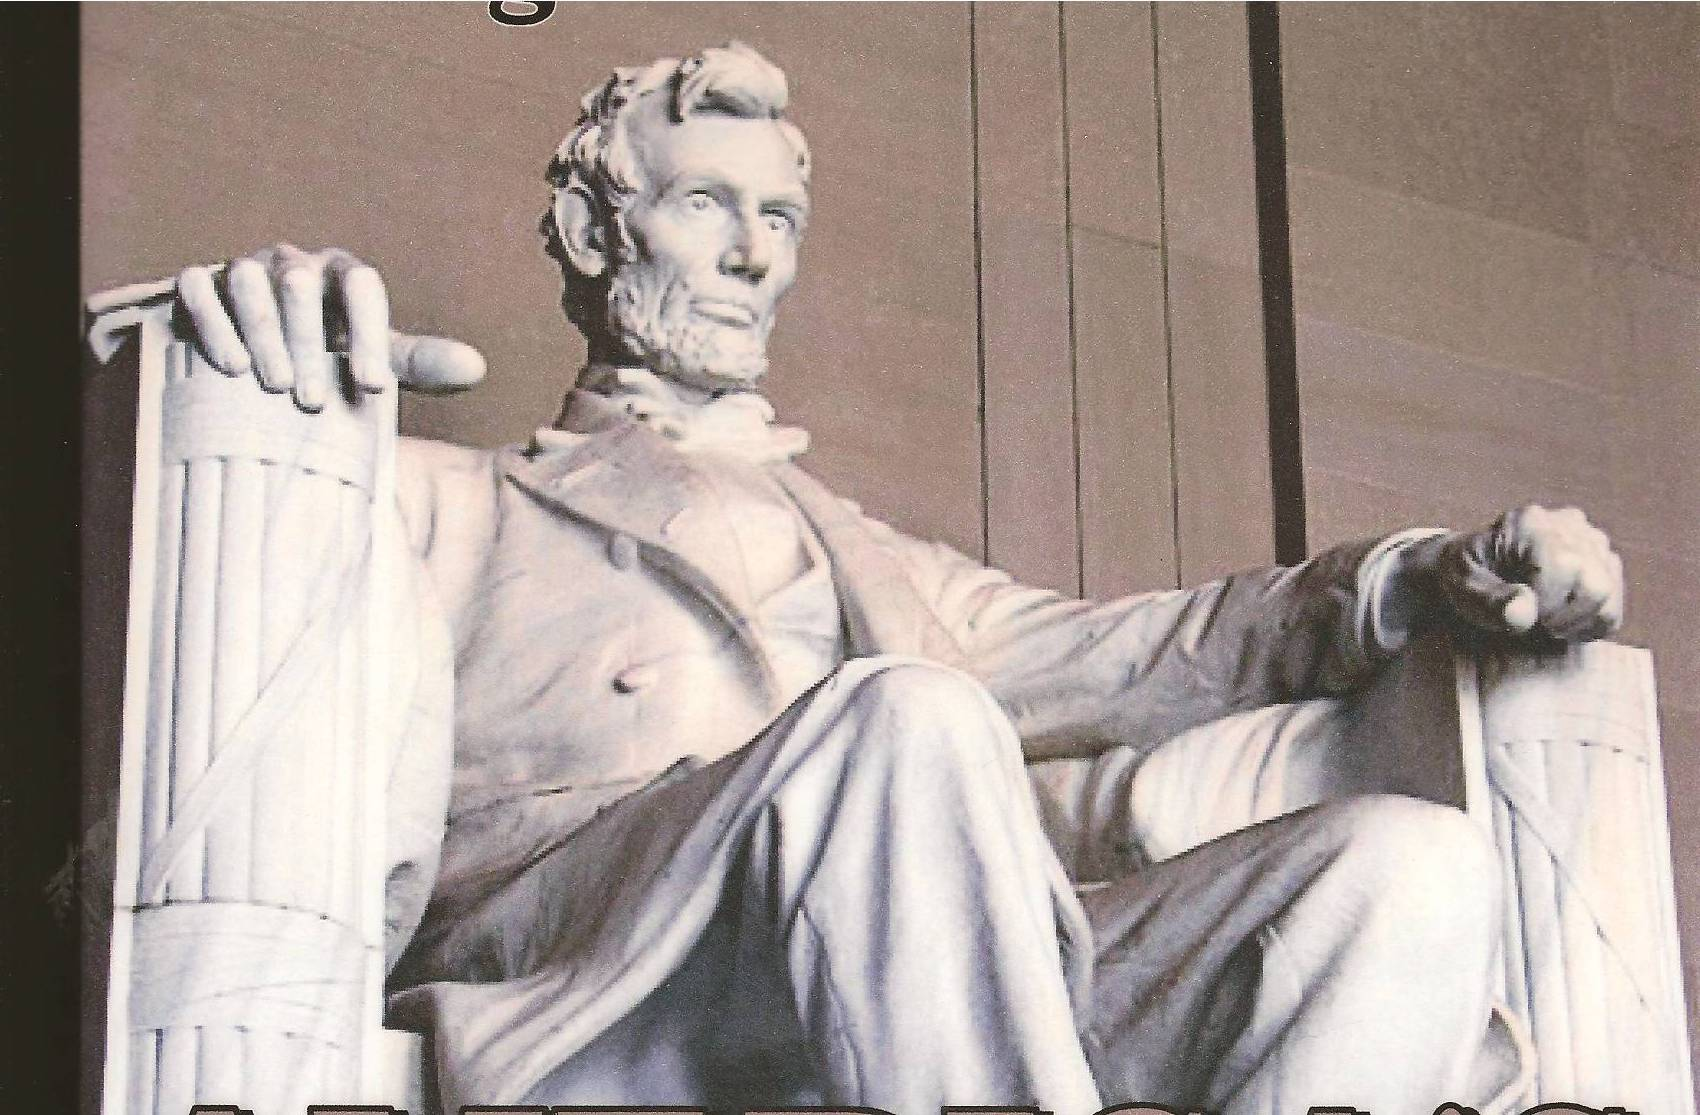
\includegraphics[width=.9\textwidth]{img/lincoln-memorial.jpg} \\
\end{frame}

\begin{frame}
    \begin{columns}[onlytextwidth]
        \column{0.5\textwidth}
            \centering
            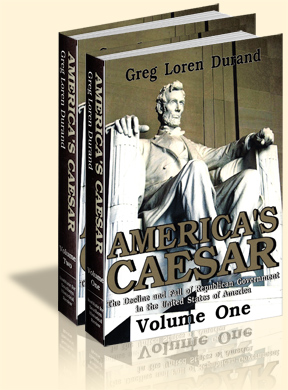
\includegraphics[width=0.75\textwidth]{img/americas-caesar.png} \\

        \column{0.5\textwidth}
            \begin{block}{America's Caesar}
                The Decline and Fall of Republican Government in the United States of America
            \end{block}
    \end{columns}
\end{frame}

\begin{frame}
    \begin{columns}[onlytextwidth]
        \column{0.5\textwidth}
            \centering
            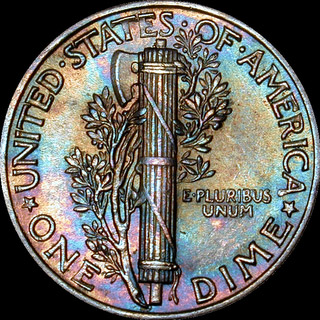
\includegraphics[width=0.75\textwidth]{img/dime-usa-fasces-2.jpg} \\
            1916 - 1945 \\

        \column{0.5\textwidth}
            \centering
            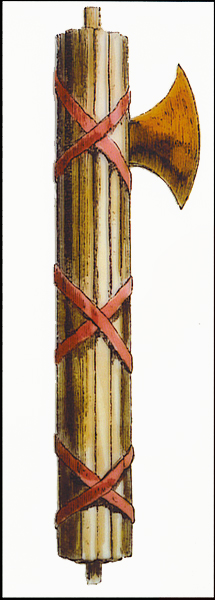
\includegraphics[height=0.55\textheight]{img/fasces-copy.jpg} \\
            Roman Law\\

    \end{columns}
\end{frame}

\begin{frame}
    \centering
    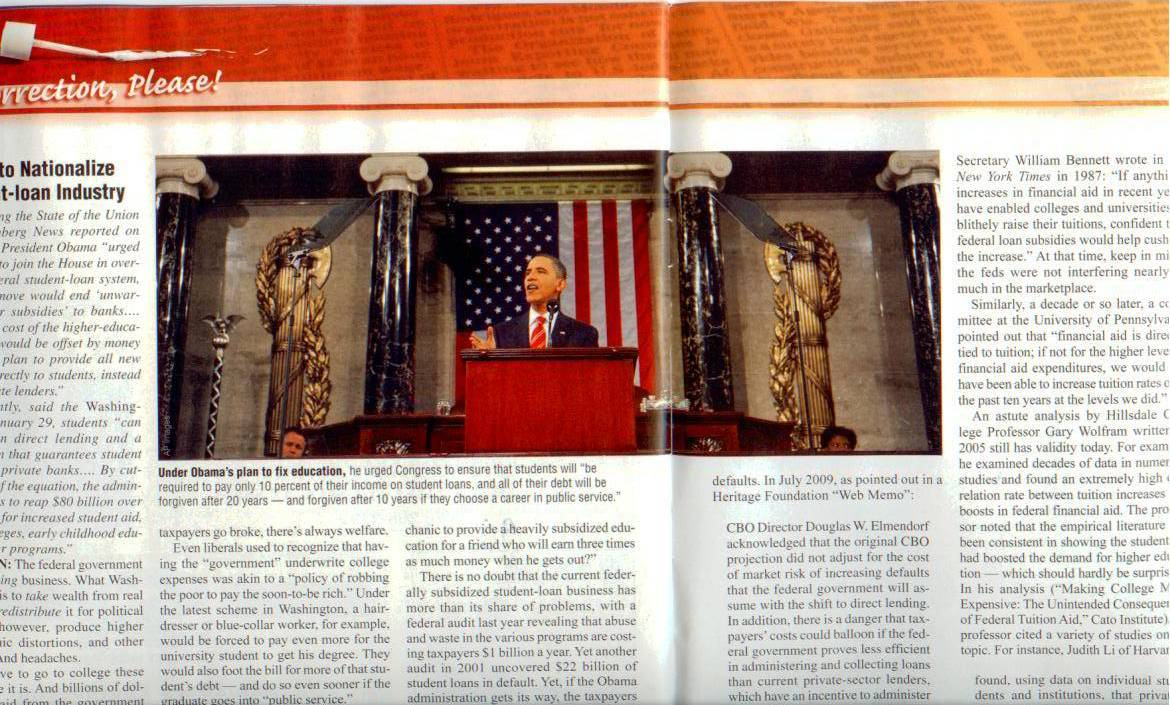
\includegraphics[width=.9\textwidth]{img/obama-fasces.jpg} \\
\end{frame}

\begin{frame}
    \centering
    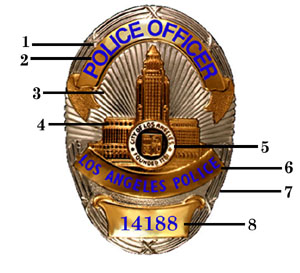
\includegraphics[height=.8\textheight]{img/fasces/badge_description.jpg} \\
    Los Angeles Police Dept. badge, developed 1939 - 1941 \\
\end{frame}
\begin{frame}
    \centering
    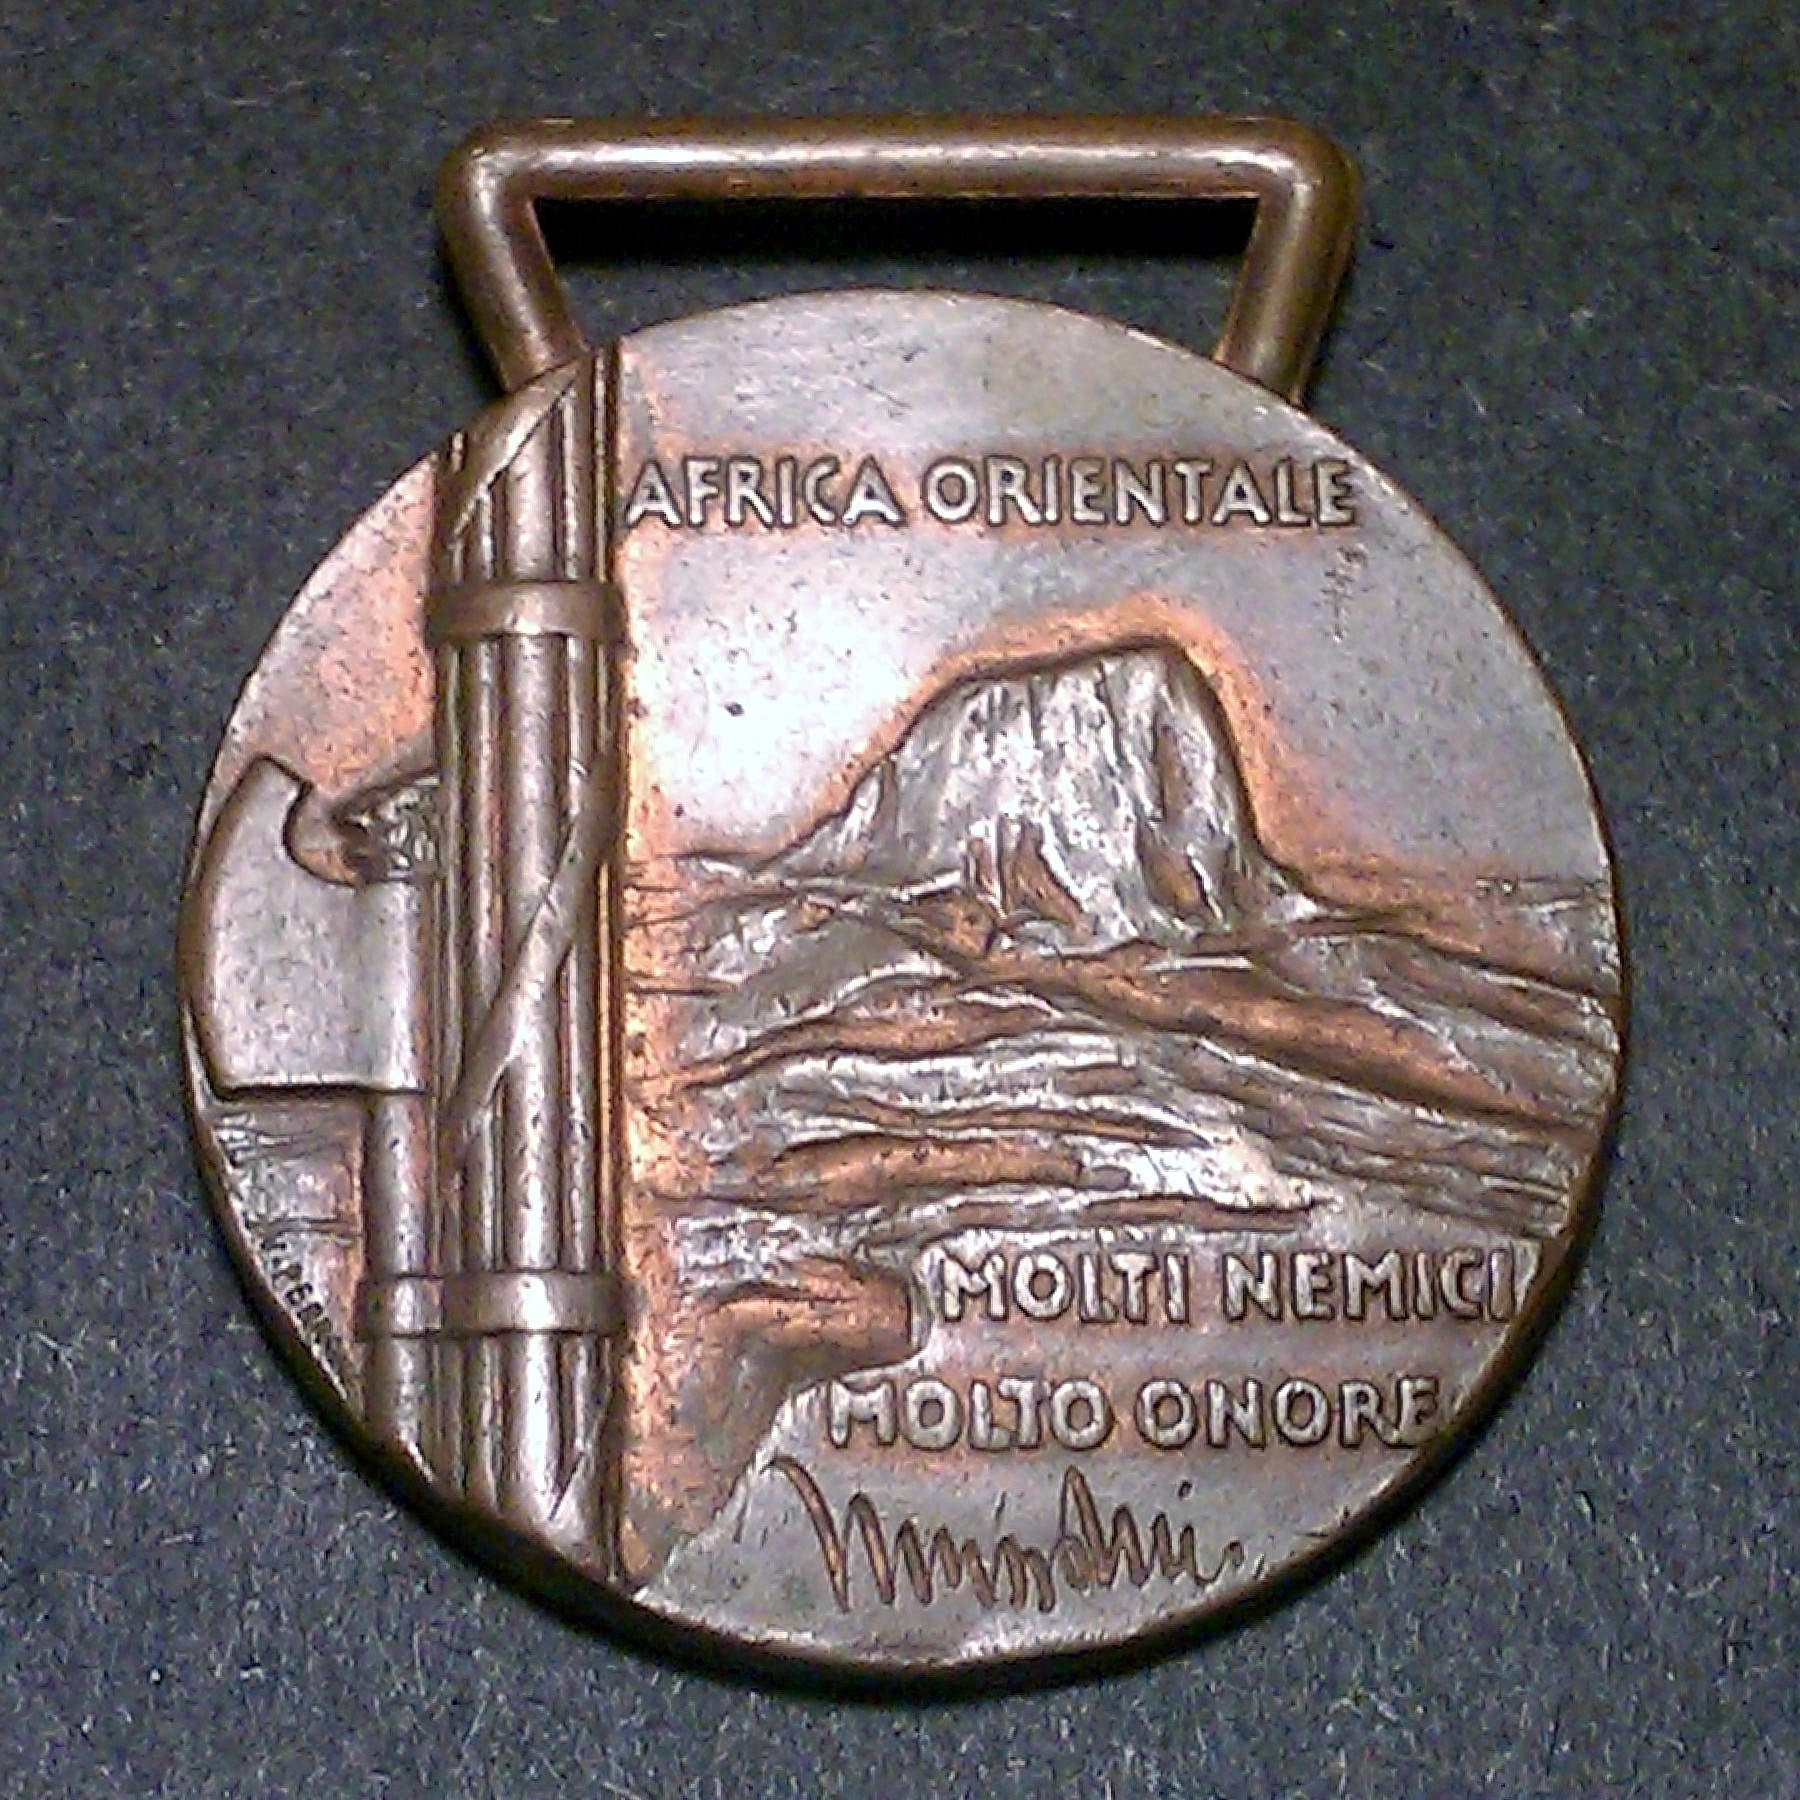
\includegraphics[height=.8\textheight]{img/fasces/coin.jpg} \\
    Italian East Africa Campaign medal, 1936 \\
\end{frame}
\begin{frame}
    \centering
    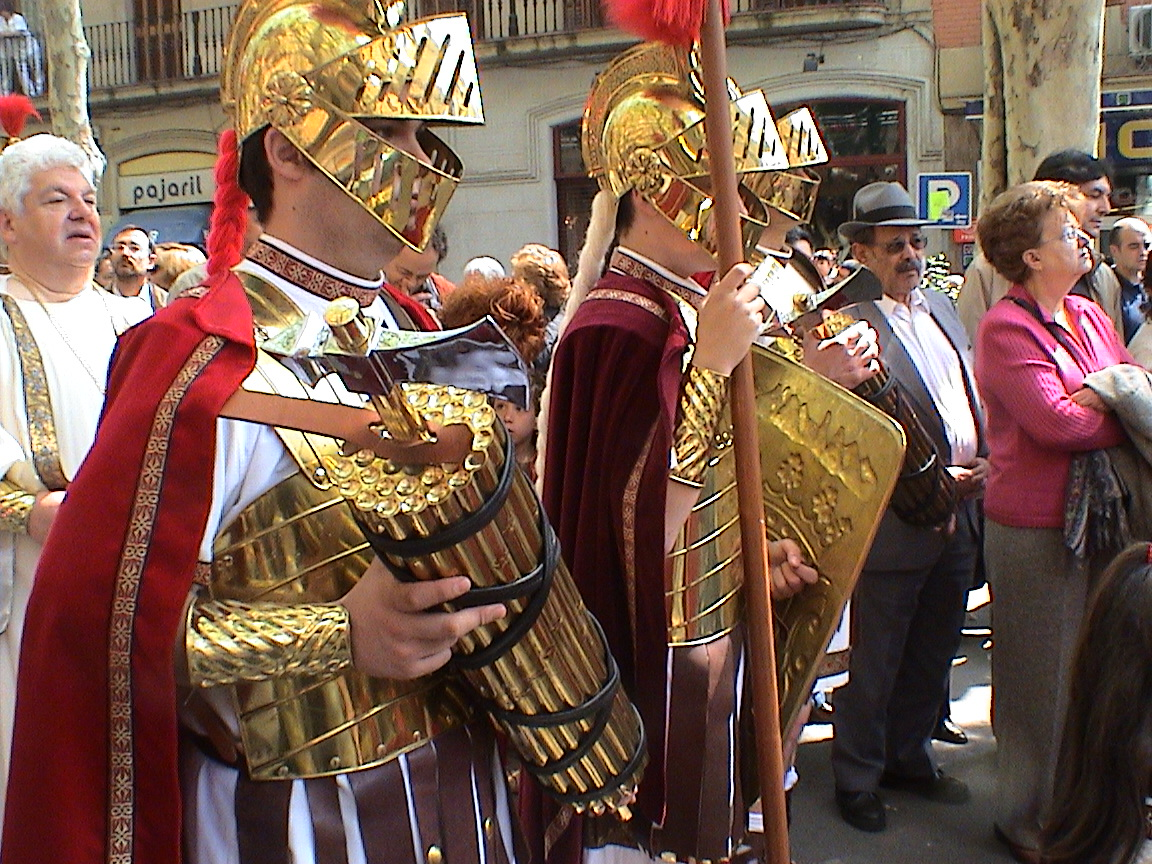
\includegraphics[width=.9\textwidth]{img/fasces/fake-fasces.jpg} \\
    Catalonia (largely autonomous Spanish province), 2006 \\
\end{frame}
\begin{frame}
    \centering
    
\includegraphics[height=.8\textheight]{img/fasces/fasces13.jpg} \\
    Adopted 1877. Text reads ``Union and Consitution''. Colorado's state website claims ``The Roman fasces is the insignia of a republican form of government\ldots The axe symbolizes authority and leadership.'' \\
\end{frame}
\begin{frame}
    \centering
    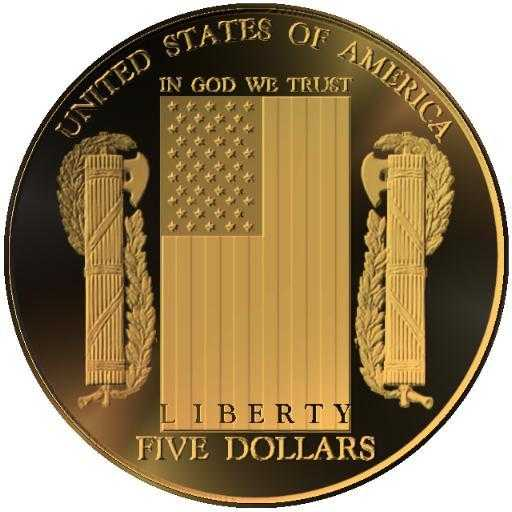
\includegraphics[height=.8\textheight]{img/fasces/fasces5coin.jpg} \\
\end{frame}
\begin{frame}
    \centering
    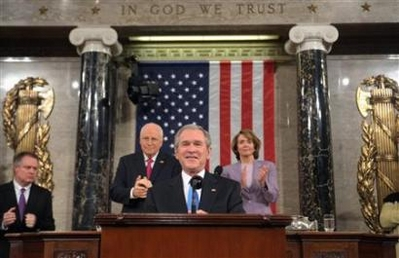
\includegraphics[width=.9\textwidth]{img/fasces/fasces_congress.jpg} \\
\end{frame}
\begin{frame}
    \centering
    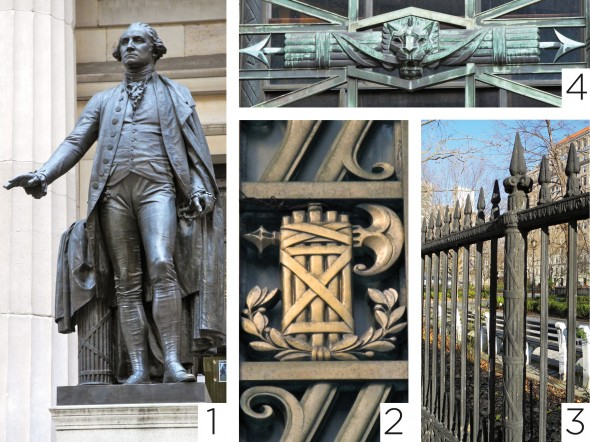
\includegraphics[width=.9\textwidth]{img/fasces/fasces-stuff.jpg} \\
    Statue by John Quincy Adams Ward, 1882.
\end{frame}
\begin{frame}
    \centering
    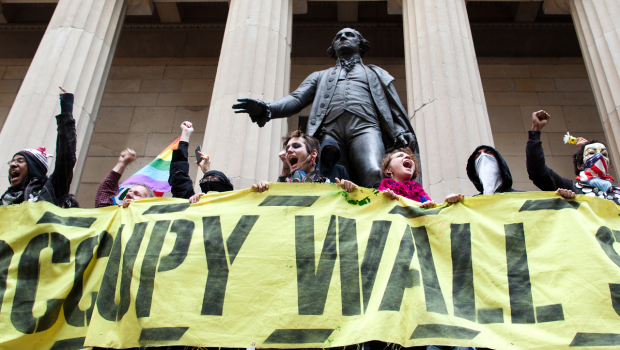
\includegraphics[width=.9\textwidth]{img/fasces/ows.jpg} \\
    Federal Hall, New York City \\
\end{frame}
\begin{frame}
    \centering
    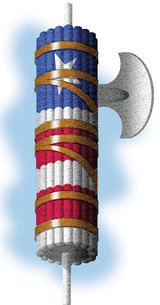
\includegraphics[height=.8\textheight]{img/fasces/flag-fasces.jpg} \\
\end{frame}
\begin{frame}
    \centering
    
\includegraphics[height=.8\textheight]{img/fasces/french-republic-symbol.png} \\
    National Symbol of France, adopted 1953. This symbol is used to represent France in the U.N. Assembly building. \\
\end{frame}
\begin{frame}
    \centering
    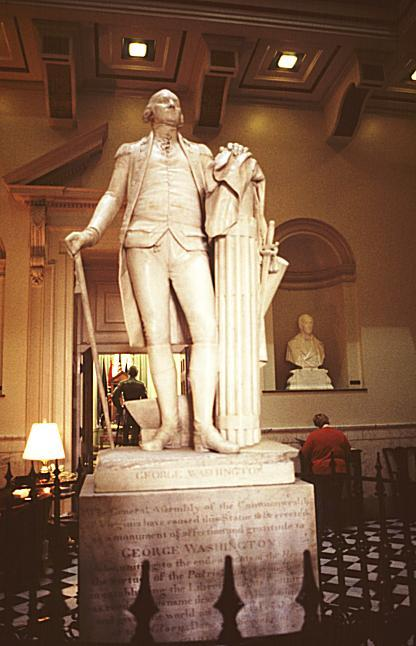
\includegraphics[height=.8\textheight]{img/fasces/houdon-front.jpg} \\
    Statue by Jean-Antoine Houdon, completed 1791. Commissioned by Virgina's legislature, and on display at Colonial Williamsburg. \\
\end{frame}
\begin{frame}
    \centering
    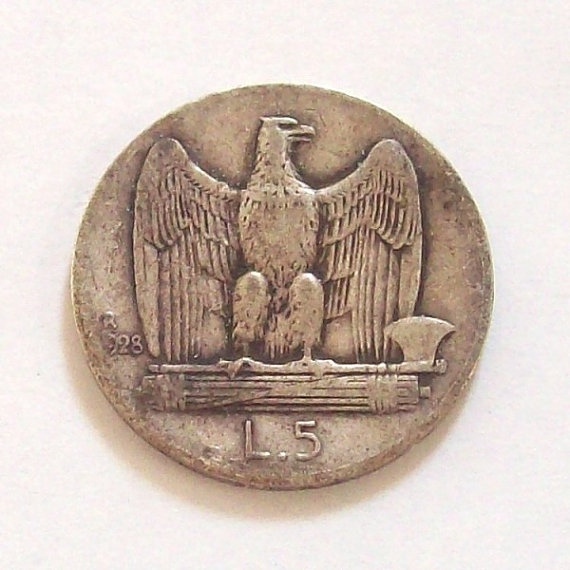
\includegraphics[height=.8\textheight]{img/fasces/italy-fasces-coin.jpg} \\
    Italian 5 lira piece, 1928 \\
\end{frame}
\begin{frame}
    \centering
    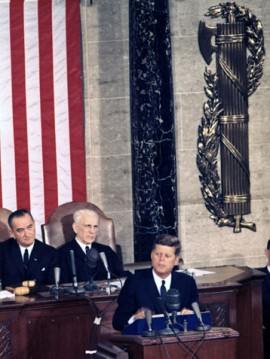
\includegraphics[height=.9\textheight]{img/fasces/jfk.jpg} \\
\end{frame}
\begin{frame}
    \centering
    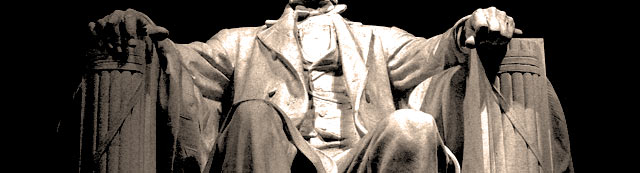
\includegraphics[width=.9\textwidth]{img/fasces/lincoln_fasces.jpg} \\
\end{frame}
\begin{frame}
    \centering
    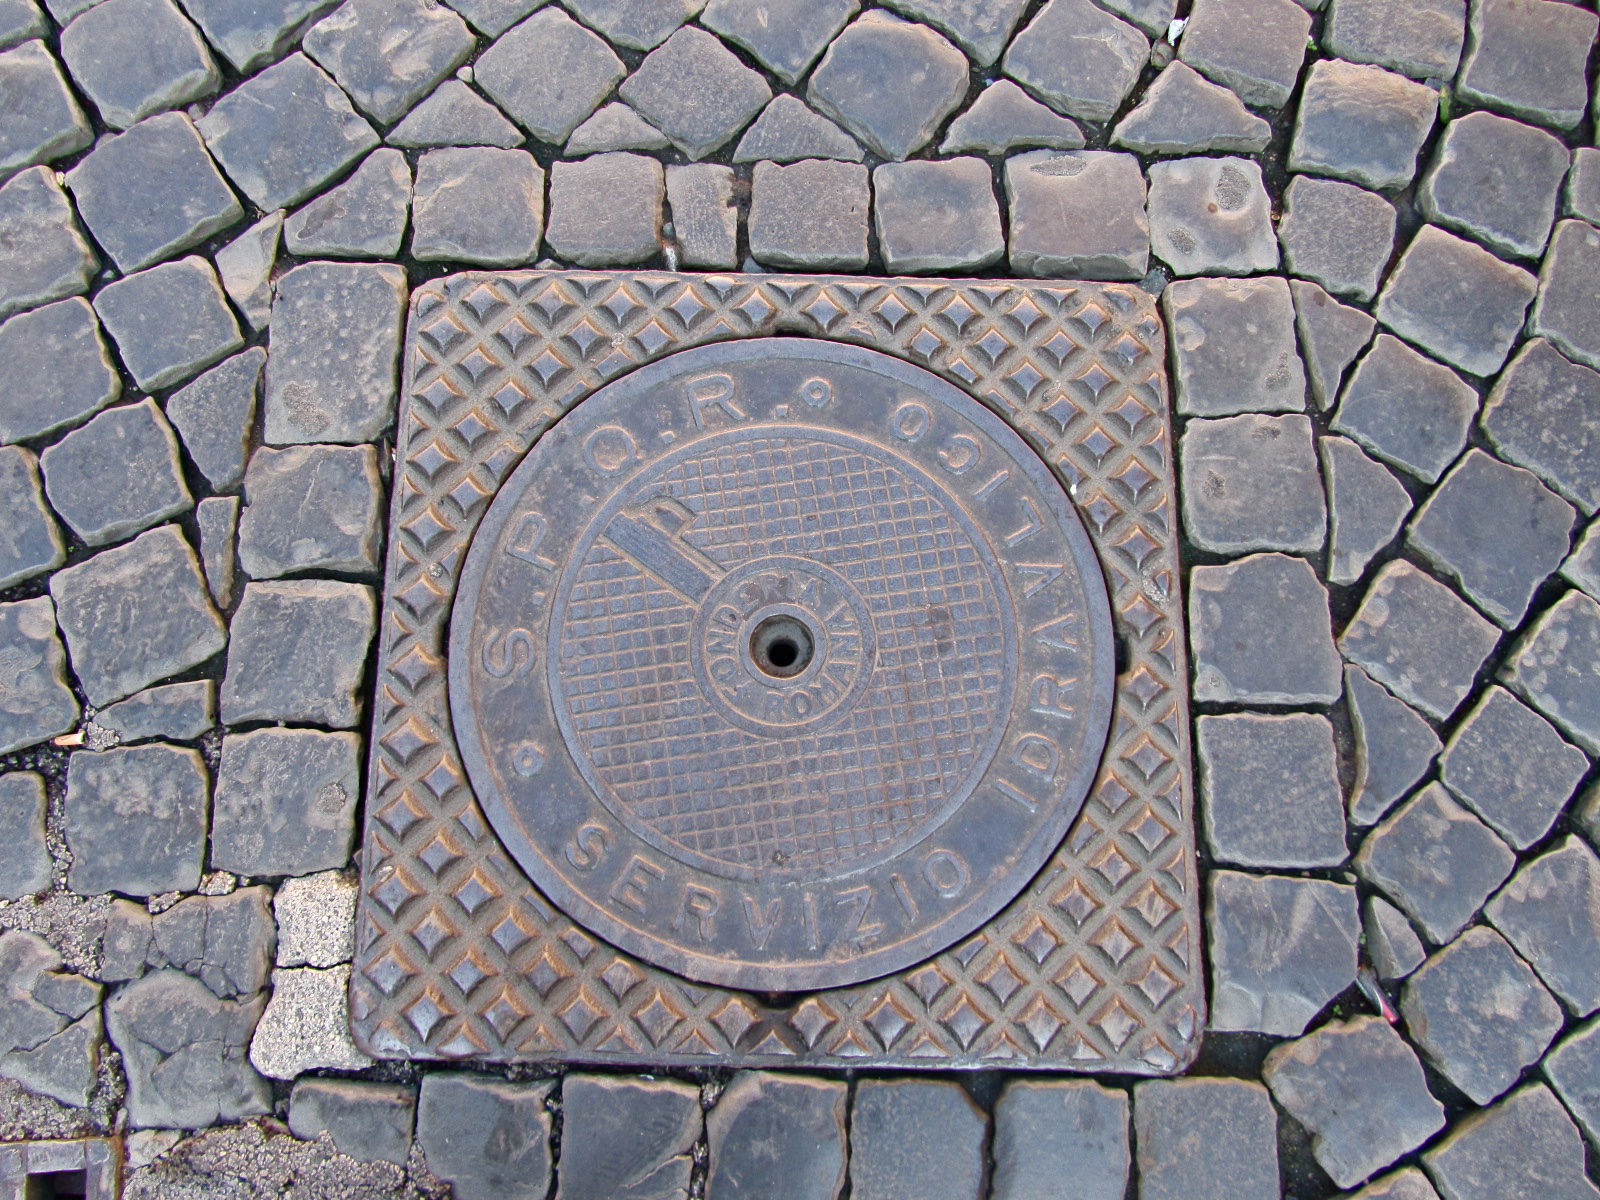
\includegraphics[width=.9\textwidth]{img/fasces/manhole.JPG} \\
\end{frame}
\begin{frame}
    \centering
    
\includegraphics[height=.8\textheight]{img/fasces/mp.jpg} \\
\end{frame}
\begin{frame}
    \centering
    
\includegraphics[height=.8\textheight]{img/fasces/tax-court.png} \\
    The Tax Court took on its present form in 1969 \\
\end{frame}
\begin{frame}
    \centering
    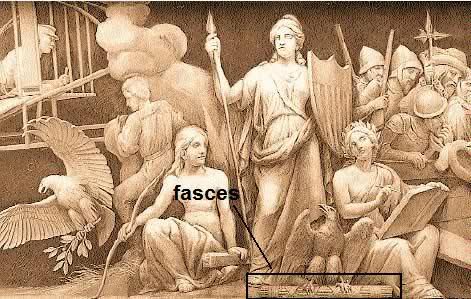
\includegraphics[height=.8\textheight]{img/fasces/teut1.jpg} \\
    Detail of frieze in the U.S. Capitol rotunda. The frieze was designed in 1859 and begun in 1877, but wasn't fully complete until 1953. \\
\end{frame}
\begin{frame}
    \centering
    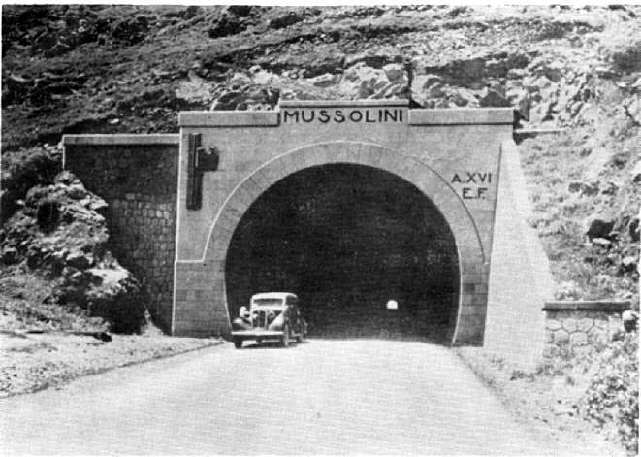
\includegraphics[width=.9\textwidth]{img/fasces/tunnel.jpg} \\
\end{frame}
\begin{frame}
    \centering
    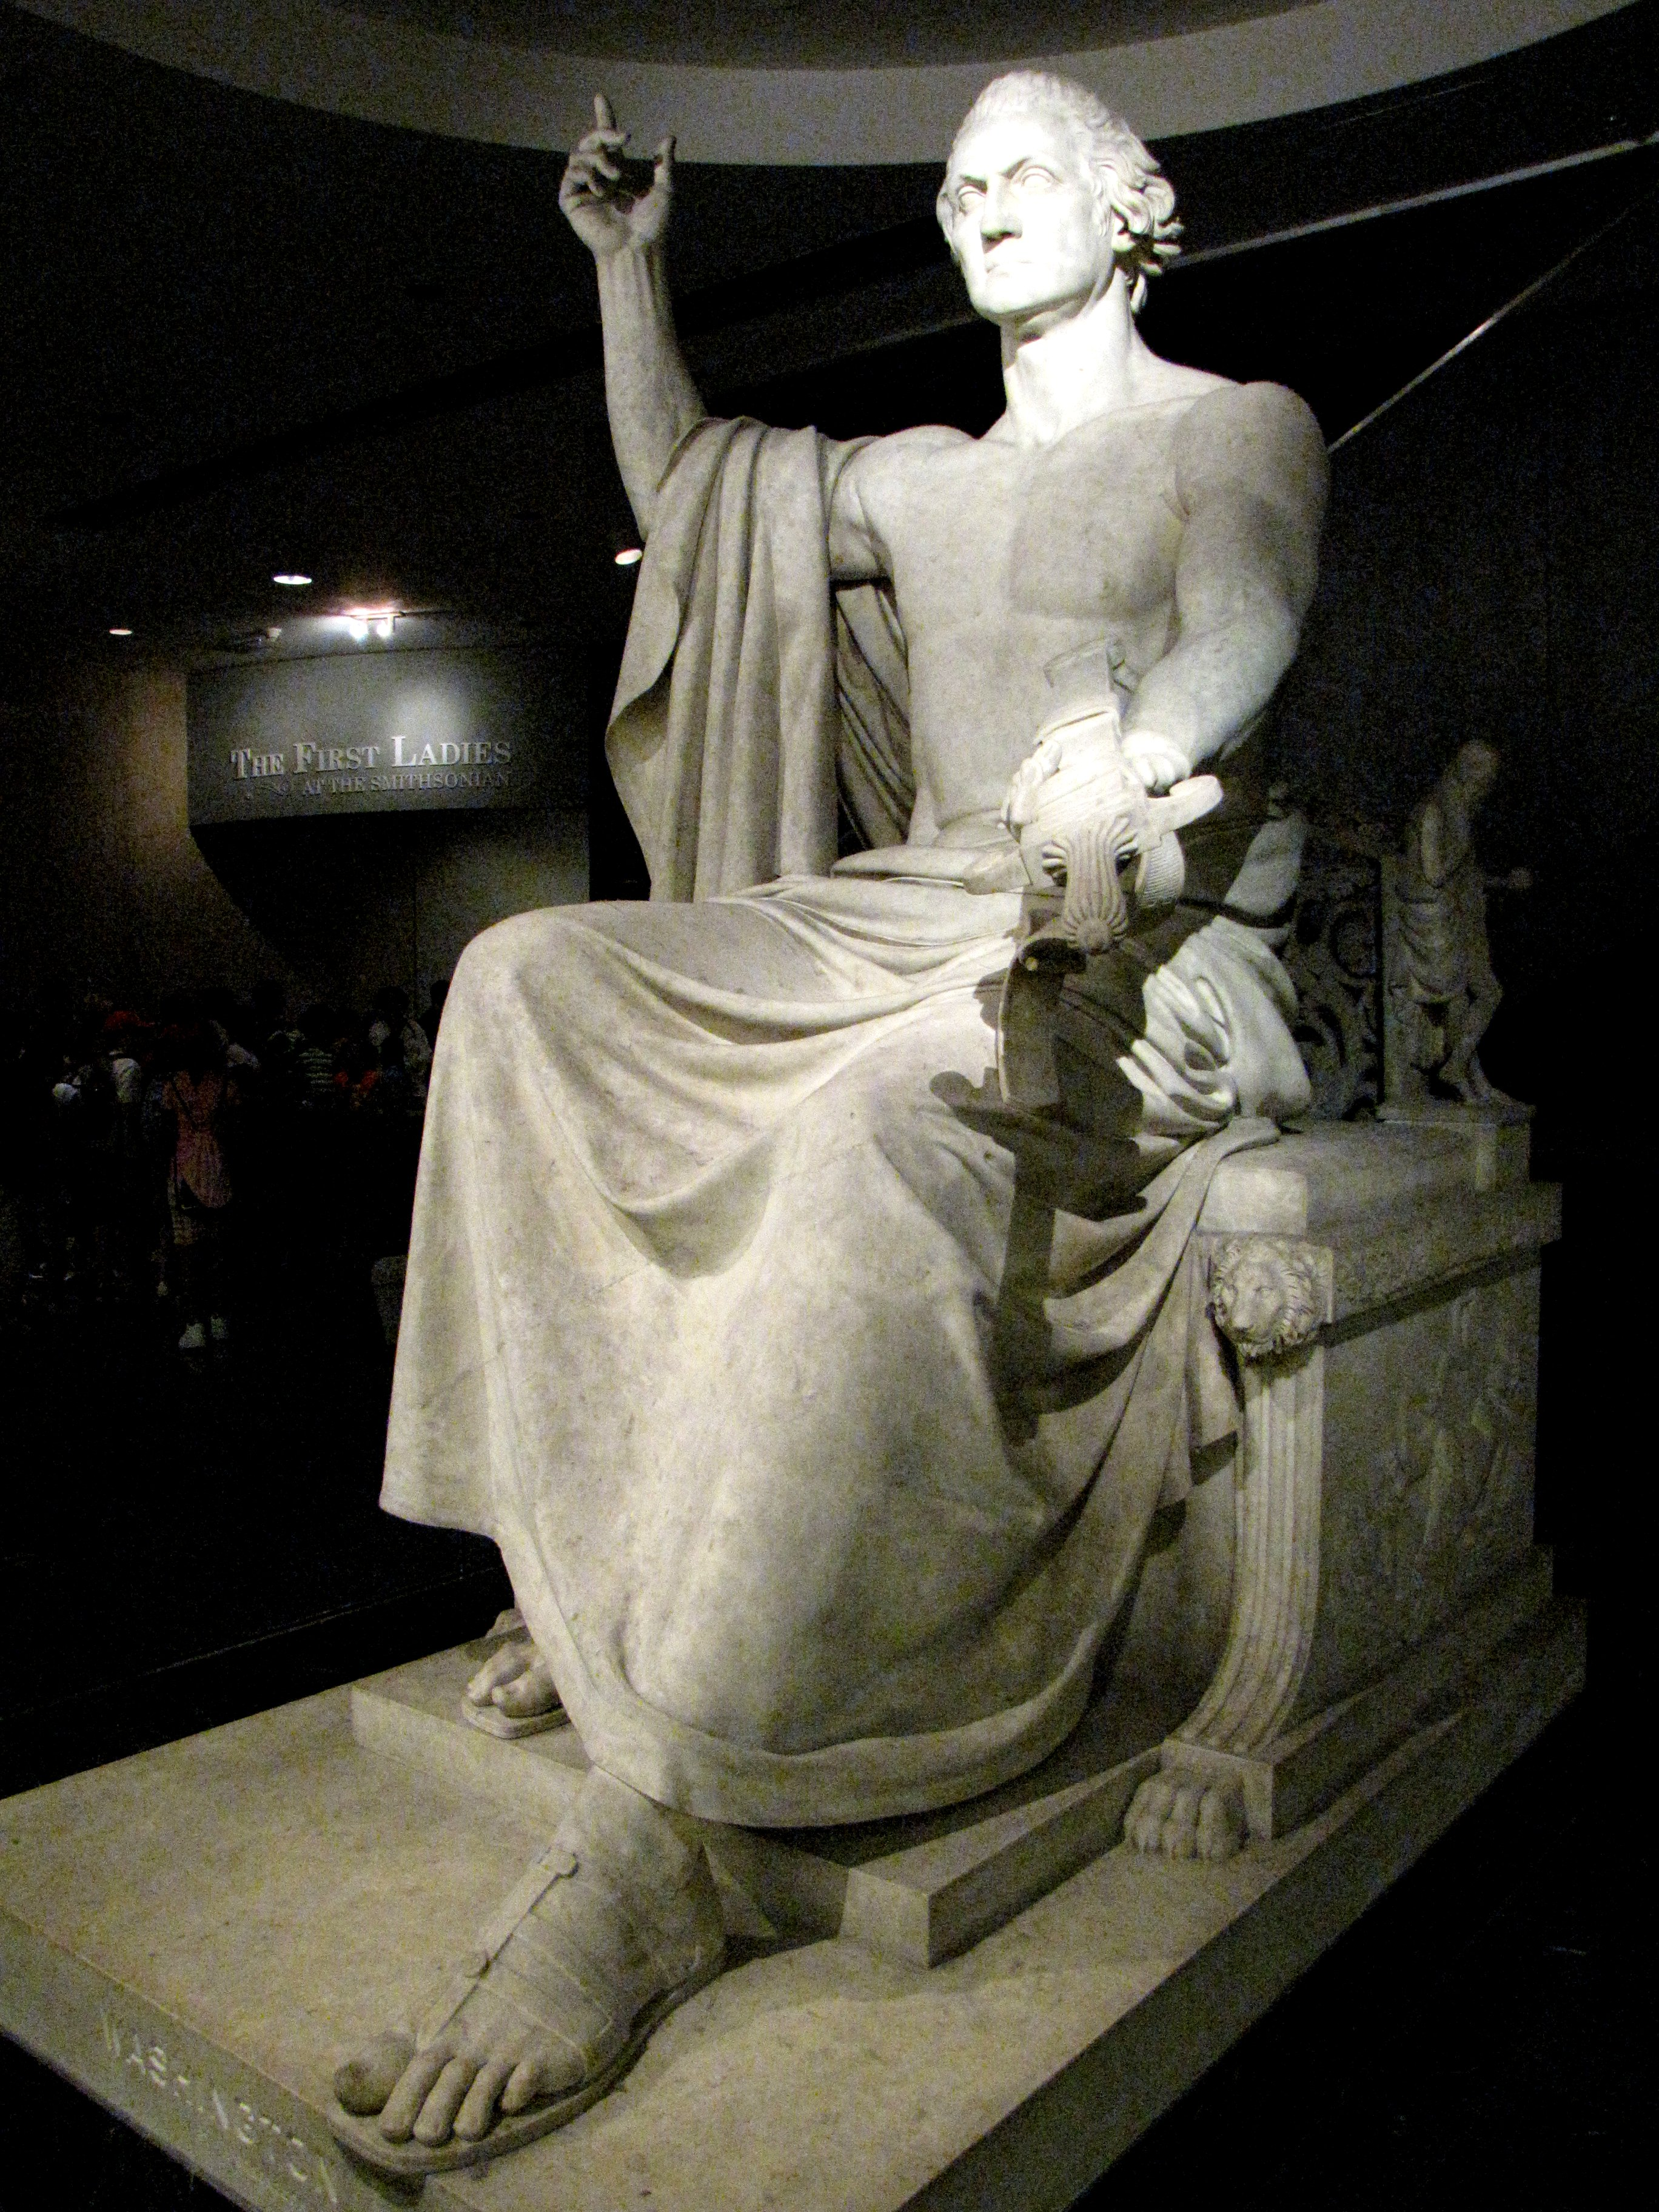
\includegraphics[height=.8\textheight]{img/fasces/washington1.jpg} \\
    By Horatio Greenough, completed in 1840, and now found in the Smithsonian
    museum of American History. The base reads,``Horatio Greenough made this
    image as a great example of freedom, and will not survive without freedom
    itself.''
\end{frame}

\begin{frame}
    \centering
    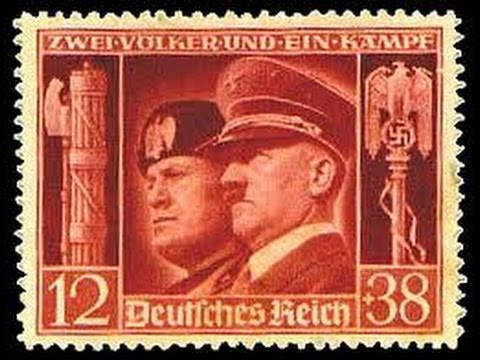
\includegraphics[width=.9\textwidth]{img/reich-stamp.png} \\
\end{frame}

\begin{frame}{Two Contending Forces}
    \begin{columns}[onlytextwidth]
        \column{0.5\textwidth}
            \begin{varblock}[0.9\textwidth]{}\huge{ \centering Sovereignty of the National Government \\}\end{varblock}

        \column{0.5\textwidth}
            \begin{varblock}[0.9\textwidth]{}\huge{ \centering Sovereignty of the individual States \\}\end{varblock}
    \end{columns}
    \textbf{\huge{ \color{red}
        \Put(155,120){v.}
    }}
\end{frame}

\begin{frame}
    \centering
    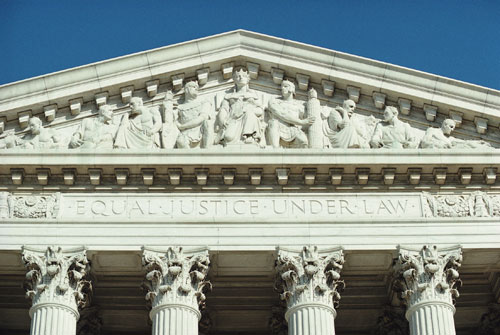
\includegraphics[width=.9\textwidth]{img/supremecourtfasces.jpg} \\
    \large{ Front of the Supreme Court building } \\
\end{frame}

\begin{frame}
    \centering
    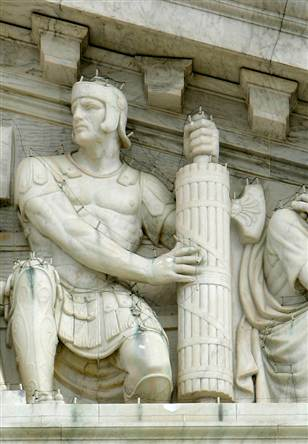
\includegraphics[height=.85\textheight]{img/fasces_west_supcourt.jpg} \\
    \large{ On November 28, 2008, 172 pounds of this facade fell four stories to land on the steps of the court } \\
\end{frame}

\begin{frame}
    \centering
    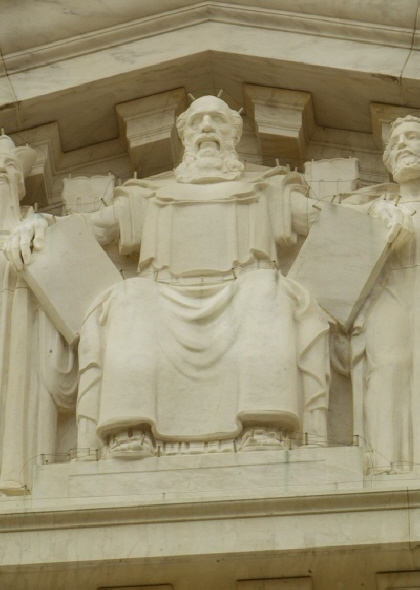
\includegraphics[height=.9\textheight]{img/moses_east_supcourt.jpg} \\
    \large{ Rear of the Supreme Court building } \\
\end{frame}

\begin{frame}
    \centering
    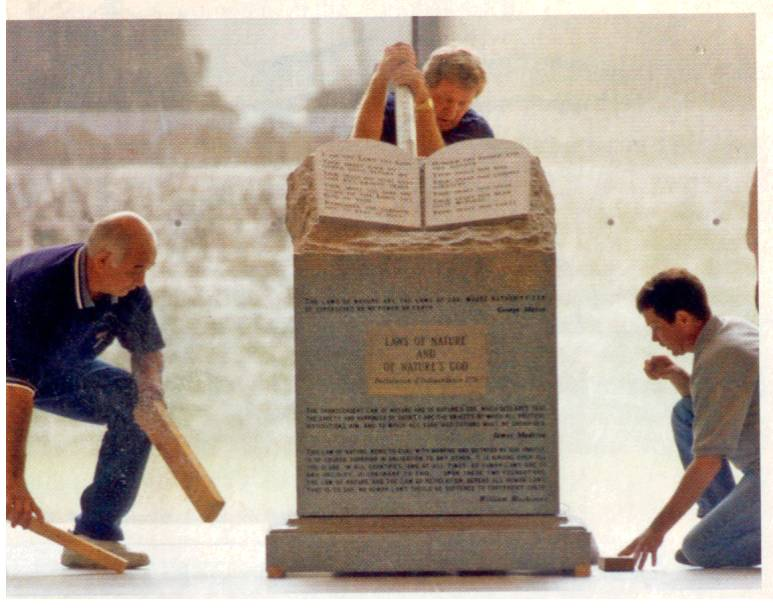
\includegraphics[width=.9\textwidth]{img/10-commandments.jpg} \\
\end{frame}

\frame{\centering 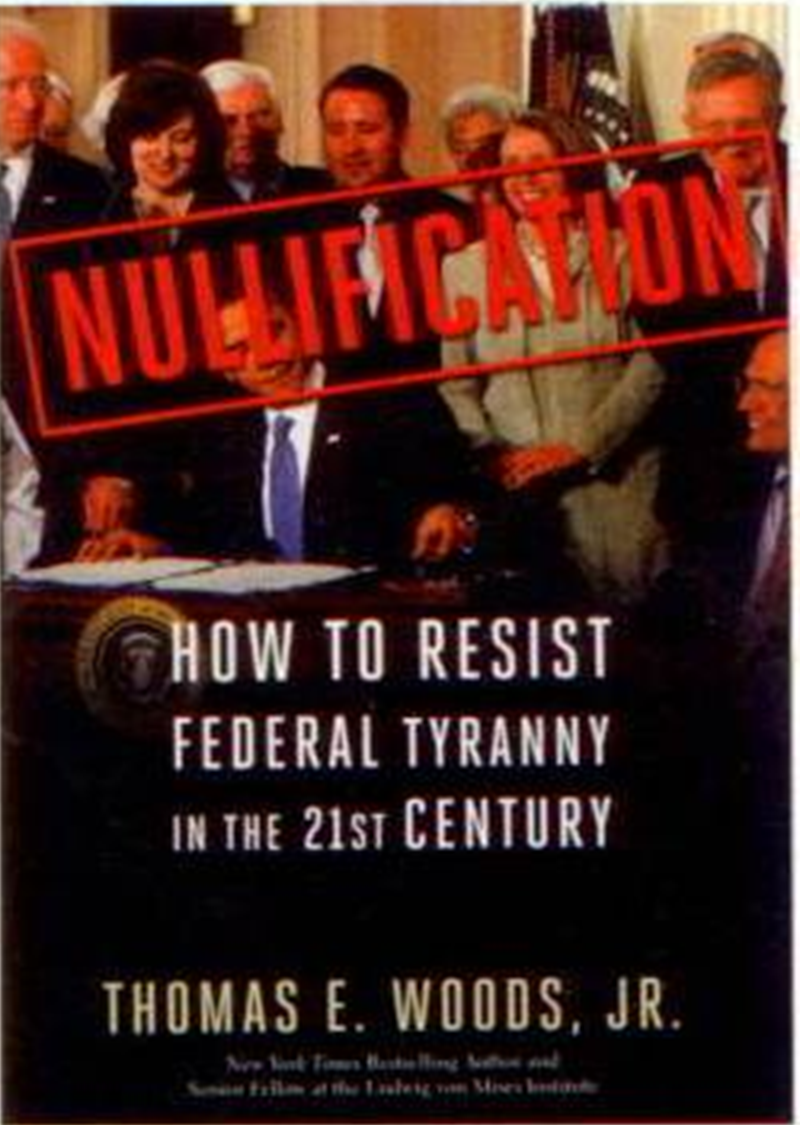
\includegraphics[keepaspectratio,width=\textwidth,height=\textheight]{img/nullification.png} \\ }
\end{document}
